\chapter{Actionable Approximations of the Truth}\label{s:pck}

\begin{objectives}

\item Explain what pedagogical content knowledge (PCK) is and why it's
  important.

\item Explain what the ``superbug'' in novice programming is, and at
  least two other misconceptions novices often have.

\item Describe what blocks-based programming tools are and why they
  are easier for novices to learn than text-based systems.

\item Describe the effects that error messages, variable naming, and
  visualization have on novices' performance.

\item Summarize the effectiveness of various intervention strategies
  on novice learning.

\end{objectives}

Every instructor needs three things:

\begin{itemize}

\item \glossref{g:content-knowledge}{content knowledge}, such as how
  to program;

\item \glossref{g:general-pedagogical-knowledge}{general pedagogical
  knowledge}, such as an understanding of the psychology of learning;
  and

\item \glossref{g:pedagogical-content-knowledge}{pedagogical
  content knowledge} (PCK), which is the domain-specific knowledge of
  how to teach a particular concept to a particular audience.

\end{itemize}

In computing, PCK includes things like what examples to use when
teaching how parameters are passed to a function, or what
misconceptions about nesting HTML tags are most common.  This chapter
summarizes some results from research into teaching and learning
programming that will add to your store of PCK.

Computing education research is still a young discipline: while the
American Society for Engineering Education was founded in 1893, and
the National Council of Teachers of Mathematics in 1920, the Computer
Science Teachers Association didn't exist until 2005.  The simple
truth is that we don't know as much about how people learn to program
as we do about how they learn to read, play a sport, or do basic
arithmetic.  However, conferences like
\href{http://sigcse.org/}{SIGCSE},
\href{http://iticse.acm.org/}{ITiCSE} and
\href{https://icer.hosting.acm.org}{ICER} are delivering an
ever-increasing stream of rigorous, insightful studies with practical
application.  (For those interested in methods these studies rely on,
\cite{Ihan2016} summarizes the ones used most often.)

As with all research, though, some caution is required to interpret
these results.  Most studies look at school children and university
undergraduates, both because those are the populations that
researchers have easiest access to \cite{Henr2010} and because those
are the ages at which people most often learn to program; less is
known about adults learning to program in free-range settings.

Theories may change as more and better data becomes available, so if
this was an academic treatise, it would preface most claims with
statements like, ``Research may seem to indicate that{\ldots}''
However, since actual teachers in actual classrooms have to make
decisions regardless of whether research has clear answers yet or not,
this chapter presents actionable approximations of the truth rather
than nuanced perhapses.

\begin{callout}{Jargon}

  Like any specialty, computing education research has its jargon.
  The term \glossref{g:cs1}{CS1} refers to an introductory
  semester-long programming course in which learners meet variables,
  loops, and functions for the first time, while \glossref{g:cs2}{CS2}
  refers to a second course that covers basic data structures like
  stacks and queues.  The term \glossref{g:cs0}{CS0} is also now being
  used to refer to an introductory course for people without any prior
  experience who aren't intending to continue with computing (at least
  not right away).

  A CS1 course is often useful for undergraduates in other
  disciplines; a CS2 course designed for computer science learners is
  usually less relevant for artists, ecologists, and other
  \glossref{g:end-user-programmer}{end-user programmers}, but is
  sometimes the only next step available at their institution.  Full
  definitions for these terms and others can be found in the
  \href{https://www.acm.org/education/curricula-recommendations}{ACM
    Curriculum Guidelines}.

\end{callout}

\section{How Do Novices Program?}\label{s:pck-programming}

\cite{Solo1984,Solo1986} pioneered the exploration of novice and
expert programming strategies.  The key finding is that experts know
both ``what'' and ``how'', i.e., they understand what to put into
programs \emph{and} they have a set of patterns or plans to guide
their construction.  Novices lack both, but most teachers focus solely
on the former, even though bugs are often caused by not having a
strategy for solving the problem rather than to lack of knowledge
about the language.

The most important recommendation in this chapter is therefore to
\emph{show learners how to program}.  This is consistent with the work
on cognitive load theory presented in \chapref{s:load}, and
\cite{Mull2007b} is just one of many studies proving its benefits;
live coding (\secref{s:performance-live}) is effective in part because
it puts ``how'' front and center.

When demonstrating the act of programming, teachers should emphasize
the importance of small steps with frequent feedback \cite{Blik2014}.
They should also emphasize the importance of picking a plan and
sticking to it rather than making more-or-less random changes to the
program and hoping that they'll work---as \cite{Spoh1985} found,
merging plans and/or goals can yield bugs because of goals being
dropped or fragmented.

Another aspect of ``how'' that teachers should present and discuss is
the order in which code is written.  \cite{Ihan2011} describes a tool
for solving Parsons Problems.  They found that experienced programmers
often drag the method signature to the beginning, then add the
majority of the control flow (i.e., loops and conditionals), and only
then add details like variable initialization and handling of corner
cases.  This out-of-order authoring is foreign to novices, who read
and write code in the order it's presented on the page; again, one of
the benefits of live coding (\secref{s:performance-live}) is that it
gives them a chance to see the sequence that more advanced programmers
actually use.

\subsection*{Roles of Variables}

One body of work that I have found very useful in teaching programming
plans to novices is the collection of single-variable design patterns
in \cite{Kuit2004,Byck2005,Saja2006}.  labelling the parts of novices'
programs gives them a vocabulary to think with and a set of
programming plans for constructing code of their own.  The patterns
are listed on the \href{http://saja.kapsi.fi/var\_roles/}{Roles of
  Variables website}, which also includes examples of each:

\begin{description}

\item[Fixed value:] A data item that does not get a new proper value
  after its initialization.

\item[Stepper:] A data item stepping through a systematic, predictable
  succession of values.

\item[Walker:] A data item traversing in a data structure.

\item[Most-recent holder:] A data item holding the latest value
  encountered in going through a succession of unpredictable values,
  or simply the latest value obtained as input.

\item[Most-wanted holder:] A data item holding the best or otherwise
  most appropriate value encountered so far.

\item[Gatherer:] A data item accumulating the effect of individual
  values.

\item[Follower:] A data item that gets its new value always from the
  old value of some other data item.

\item[One-way flag:] A two-valued data item that cannot get its
  initial value once the value has been changed.

\item[Temporary:] A data item holding some value for a very short time
  only.

\item[Organizer:] A data structure storing elements that can be
  rearranged.

\item[Container:] A data structure storing elements that can be added
  and removed.

\end{description}

\section{How Do Novices Debug and Test?}\label{s:pck-debug}

A decade ago, \cite{McCa2008} wrote, ``It is surprising how little
page space is devoted to bugs and debugging in most introductory
programming textbooks.''  Little has changed since: there are hundreds
of books on compilers and operating systems, but only a handful about
debugging, and I have never seen an undergraduate course on the
subject.  One reason is that debugging is a ``how'' rather than a
``what''; again, one of the benefits of live coding is that it gives
teachers a chance to demonstrate the process in a way that textbooks
cannot (\secref{s:performance-live}).

\cite{List2004,List2009} found that many novices struggled to predict
the output of short pieces of code and to select the correct
completion of the code from a set of possibilities when told what it
was supposed to do.  More recently, \cite{Harr2018} found that the gap
between being able to trace code and being able to write it has
largely closed by CS2, but that novices who still have a gap (in
either direction) are likely to do poorly in the course.

Our second recommendation is therefore to \emph{teach novices how to
  debug}.  \cite{Fitz2008,Murp2008} found that good debuggers were
good programmers, but not all good programmers were good at debugging.
those who were used a symbolic debugger to step through their
programs, traced execution by hand, wrote tests, and re-read the spec
frequently, which are all teachable habits. However, tracing execution
step by step was sometimes used ineffectively: for example, a novice
might put the same \texttt{print} statement in both parts of an
\texttt{if}-\texttt{else}.  Novices would also comment out lines that
were actually correct as they tried to isolate a problem; teachers can
make both of these mistakes deliberately, point them out, and correct
them to help novices get past them.

Teaching novices how to debug can also help make classes easier to
manage.  \cite{Alqa2017} found that learners with more experience
solved debugging problems significantly faster, but times varied
widely: 4--10 minutes was a typical range for individual exercises,
which means that some learners need 2--3 times longer than others to
get through the same exercises.  Teaching the slower learners what the
faster ones are doing will help make the group's overall progress more
uniform.

Debugging depends on being able to read code, which multiple studies
have shown is the single most effective way to find bugs
\cite{Basi1987,Keme2009,Bacc2013}.  The code quality rubric developed
in \cite{Steg2014,Steg2016a}, which is online at \cite{Steg2016b}, is
a good checklist of things to look for, though it is best presented in
chunks rather than all at once.

Having learners read code and summarize its behavior is a good
exercise (\secref{s:individual-strategies}), but often takes too long
to be practical in class.  Having them predict a program's output just
before it is run, on the other hand, helps reinforce learning
(\secref{s:classroom-practices}) and also gives them a natural moment
to ask ``what if'' questions.  Instructors or learners can also trace
changes to variables as they go along (\figref{f:pck-sketch}), which
\cite{Cunn2017} found was effective.

\begin{figure}
\centering
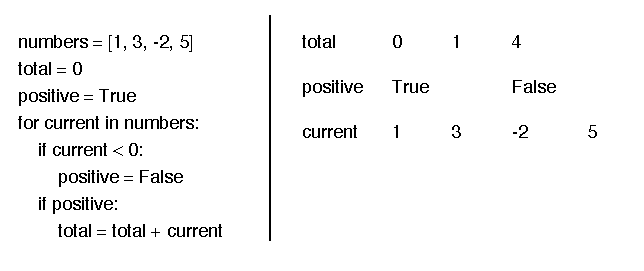
\includegraphics{../docs/fig/sketching-variables.pdf}
\caption{Tracing the Values of Variables)}
\label{f:pck-sketch}
\end{figure}

When it comes to testing, novices seem just as reluctant to do it as
professional programmers.  There's no doubt it's
valuable---\cite{Cart2017} found that high-performing novices spent a
lot of time testing, while low performers spent much more time working
on code with errors---and many instructors require learners to write
tests for assignments.  The question is, how well do they do this?

One answer comes from \cite{Bria2015}, which scored learners' programs
by how many teacher-provided test cases those programs passed, and
conversely scores test cases written by learners according to how many
deliberately-seeded bugs they caught.  They found that novices' tests
often have low coverage (i.e., they don't test most of the code) and
that they often test many things at once, which makes it hard to
pinpoint the causes of errors.

Another answer comes from \cite{Edwa2014b}, which looked at all of the
bugs in all novices' code submissions combined and identified those
detected by the novices' test suite.  They found that novices' tests
only detected an average of 13.6\% of the faults present in the entire
program population.  What's more, 90\% of the novices' tests were very
similar, which indicates that novices mostly write tests to confirm
that code is doing what it's supposed to rather than to find cases
where it isn't.

One approach to teaching better testing practices is to define a
programming problem by providing a set of tests to be passed rather
than through a written description (\secref{s:exercises-classics}).
Before doing this, though, take a moment to look at how many tests
you've written for your own code recently, and then decide whether
you're teaching what you believe people should do, or what they (and
you) actually do.

\section{What Misconceptions Do Novices Have?}\label{s:pck-misunderstand}

\chapref{s:models} explained why clearing up novices misconceptions is
just as important as teaching them strategies for solving problems.
The biggest misconception novices have---sometimes called the
``superbug'' in coding---is the belief that they can communicate with
a computer in the same way that they would with a human being, i.e.,
that the computer understands intention the way that a human being
would \cite{Pea1986}.  Our third recommendation is therefore to
\emph{teach novices that computers don't understand programs}, i.e.,
that calling a variable ``cost'' doesn't guarantee that its value is
actually a cost.

\cite{Sorv2018} presents over 40 other misconceptions that instructors
can also try to clear up, many of which are also discussed in
\cite{Qian2017}'s survey.  One is the belief that variables in
programs work the same way they do in spreadsheets, i.e., that after
executing:

\begin{verbatim}
grade = 65
total = grade + 10
grade = 80
print(total)
\end{verbatim}

\noindent
the value of \texttt{total} will be 90 rather than 75 \cite{Kohn2017}.
(This is an example of the way in which novices construct a
plausible-but-wrong mental model by making analogies.)  Other
misconceptions include:

\begin{itemize}

\item
  A variable holds the history of the values it has been assigned,
  i.e., it remembers what its value used to be.

\item
  Two objects with the same value for a \texttt{name} or \texttt{id}
  attribute are guaranteed to be the same object.

\item
  Functions are executed as they are defined, or are executed in the
  order in which they are defined.

\item
  A \texttt{while} loop's condition is constantly evaluated, and the
  loop stops as soon as it becomes false.  Conversely, the conditions
  in \texttt{if} statements are also constantly evaluated, and their
  statements are executed as soon as the condition becomes true, no
  matter where the flow of control is at the time.

\item
  Assignment moves values, i.e., after \texttt{a = b}, the variable
  \texttt{b} is empty.

\end{itemize}

Instead of looking directly at misconceptions, \cite{Muhl2016}
analyzed 350 concept maps and compared those who had done a CS course
and those who had not.  Unsurprisingly, they found that the maps drawn
by those with previous experience looked more like the maps experts
would draw, but the details highlighted what exactly learners were
taking away from their lessons: ``program'' was a central concept in
both sets of concept maps, but the next most central for those with
prior exposure were ``class'' (in the object-oriented sense) and
``data structure'', while for those without, they were ``processor''
and ``data''.

\section{What Mistakes Do Novices Make?}\label{s:pck-mistakes}

The mistakes novices make can tell us what to prioritize in our
teaching, but it turns out that most teachers don't know how common
different kinds of mistakes actually are.  The largest study of this
is \cite{Brow2017}'s study of novice Java programs, which found that
Mismatched quotes and parentheses are the most common type of error,
but also the easiest to fix, while some mistakes (like putting the
condition of an \texttt{if} in \texttt{\{\}} instead of \texttt{()})
are most often made only once.  Unsurprisingly, mistakes that produce
compiler errors are fixed much faster than ones that don't.

Some mistakes, however, are made many times, like invoking methods
with the wrong arguments (e.g., passing a string instead of an
integer).  One caution when reading this research is how important it
is to distinguish mistakes from work in progress: for example, an
empty \texttt{if} statement or a method that's defined but not yet
used may be a sign of incomplete code rather than an error.

\cite{Brow2017} also compared the mistakes novices actually make with
what their teachers thought they made.  They found that,
``{\ldots}educators formed only a weak consensus about which mistakes
are most frequent, that their rankings bore only a moderate
correspondence to the students in the{\ldots}data, and that educators'
experience had no effect on this level of agreement.''  For example,
mistaking \texttt{=} (assignment) and \texttt{==} (equality) in loop
condition tests wasn't nearly as common as most teachers believed.

\begin{callout}{Not Just for Code}

  \cite{Park2015} collected data from an online HTML editor during an
  introductory web development course.  Nearly all learners made
  syntax errors that remained unresolved weeks into the course.  20\%
  of these errors related to the relatively complex rules that dictate
  \emph{when} it is valid for HTML elements to be nested in one
  another, but 35\% related to the simpler tag syntax determining
  \emph{how} HTML elements are nested.  (The tendency of many
  instructors to say, ``But the rules are simple,'' is a good example
  of expert blind spot discussed in \chapref{s:memory}{\ldots})

\end{callout}

\section{What Are We Teaching Them Now?}\label{s:pck-now}

Very little is known about what coding bootcamps and other free-range
initiatives teach, in part because many are reluctant to share their
curriculum.  We do know more about what is taught in schools:
\cite{Luxt2017} surveyed the topics included in introductory
programming courses, categorized their findings under a dozen
headings, and ranked them by frequency:

{\small
\begin{longtable}{lrr}
  Topic & Number of Courses & (\%) \\
  Programming Process & 90 & (87\%) \\
  Abstract Programming Thinking & 65 & (63\%) \\
  Data Structures & 41 & (40\%) \\
  Object-Oriented Concepts & 37 & (36\%) \\
  Control Structures & 34 & (33\%) \\
  Operations \& Functions & 27 & (26\%) \\
  Data Types & 24 & (23\%) \\
  Input/Output & 18 & (17\%) \\
  Libraries & 15 & (15\%) \\
  Variables \& Assignment & 14 & (14\%) \\
  Recursion & 10 & (10\%) \\
  Pointers \& Memory Management & 5 & (5\%) \\
\end{longtable}
}

This paper also showed how concepts are connected.  For example, it's
impossible to explain how operator precedence works without first
explaining a few operators, and difficult to explain those in a
meaningful way without first introducing variables (because otherwise
you're comparing constants in expressions like \texttt{5{\textless}3},
which is confusing).

Similarly, \cite{Rich2017} reviewed a hundred articles to find
learning trajectories for computing classes in elementary and middle
schools, and presented results for sequencing, repetition, and
conditionals.  These are essentially collective concept maps, as they
combine and rationalize the implicit and explicit thinking of many
different educators.  \figref{f:pck-trajectory} shows the learning
trajectories for conditionals.

\begin{figure}
\centering
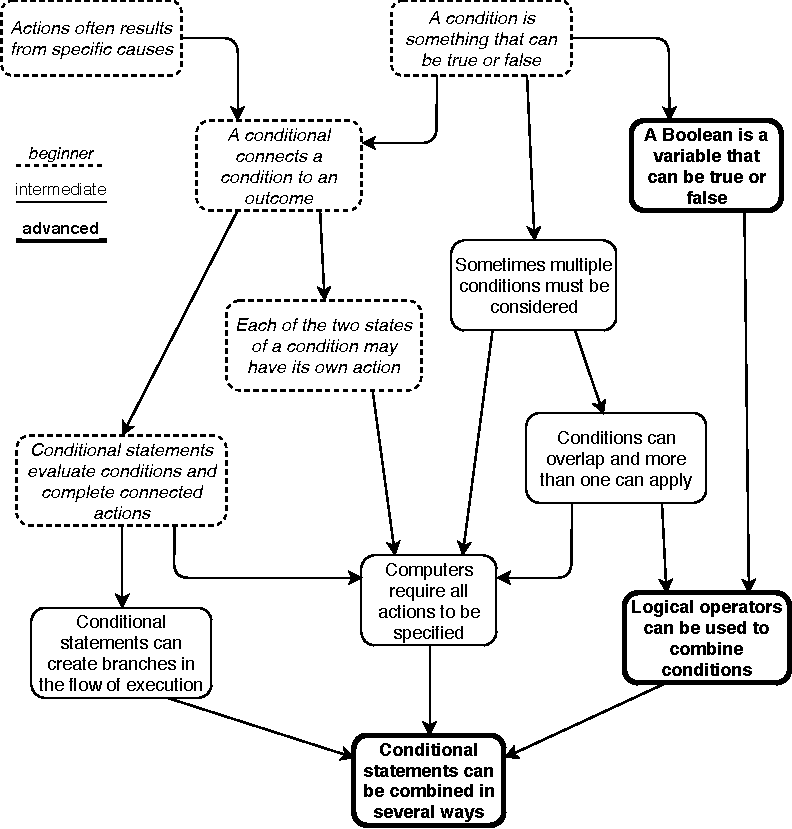
\includegraphics{../docs/fig/conditionals.pdf}
\caption{Learning Trajectory for Conditions (from \cite{Rich2017})}
\label{f:pck-trajectory}
\end{figure}

But there can be a world of difference between what instructors teach
and what learners learn, and study after study has shown that teaching
evaluations don't correlate with actual learning outcomes
\cite{Star2014,Uttl2017}.  To find out how much novices are actually
learning, we therefore have to use other measures or do direct
studies.  Taking the former approach, roughly two-thirds of
post-secondary students pass their first computing course, with some
variations depending on class size and so on, but with no significant
differences over time or based on language \cite{Benn2007a,Wats2014}.

How does prior experience affect these results?  To find out,
\cite{Wilc2018} compared the performance and confidence of novices
with and without prior programming experience in CS1 and CS2.  They
found that novices with prior experience outscored novices without by
10\% in CS1, but those differences disappeared by the end of CS2.
They also found that women with prior exposure outperformed their male
peers in all areas, but were consistently less confident in their
abilities; we will return to this issue in
\secref{s:motivation-inclusivity}.

As for direct studies of how much novices learn, \cite{McCr2001}
presented a multi-site international study, which was later replicated
by \cite{Utti2013}.  According to the first study, ``{\ldots}the
disappointing results suggest that many students do not know how to
program at the conclusion of their introductory courses.''  More
specifically, ``For a combined sample of 216 students from four
universities, the average score was 22.89 out of 110 points on the
general evaluation criteria developed for this study.''  This result
may say as much about teachers' expectations as it does about student
ability, but either way, our fourth recommendation is to \emph{measure
  and track results} in ways that can be compared over time, so that
you can tell if your lessons are becoming more or less effective.

\section{Do Languages Matter?}\label{s:pck-language}

The short answer is ``yes'': novices learn to program faster and also
learn more using blocks-based tools like Scratch
(\figref{f:pck-scratch}) that make syntax errors impossible
\cite{Wein2017b}.  And block interfaces encourage exploration in a way
that text does not; like all good tools, Scratch can be learned
accidentally \cite{Malo2010}.

Our fifth recommendation is therefore to \emph{start children and
  teens with blocks-based interfaces} before moving to text-based
systems.  The age qualification is there because Scratch
(deliberately) looks like it's meant for younger users; while
imitators like \href{https://developers.google.com/blockly/}{Blockly}
look more grown-up, it can still be hard to convince adults to take
them seriously.

\begin{figure}
\centering
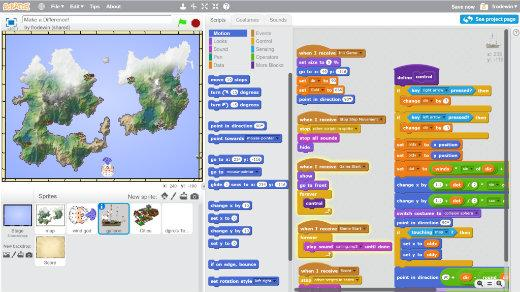
\includegraphics{../docs/fig/scratch.jpg}
\caption{Scratch (from \url{https://opensource.com/article/18/4/designing-game-scratch-open-jam})}
\label{f:pck-scratch}
\end{figure}

Scratch has probably been studied more than any other programming
tool, and we know a great deal about how it is used.  As just one
example, \cite{Aiva2016} analyzed over 250,000 Scratch projects and
found (among other things) that about 28\% of projects have some blocks
that are never called or triggered.  The authors hypothesize that
users may be using them as a scratchpad to keep bits of code they
don't (yet) want to throw away.

\cite{Grov2017,Mlad2017} studied novices learning about loops in
Scratch, Logo, and Python, and found that misconceptions about loops
are minimized when using a block-based language rather than a
text-based language.  What's more, as tasks become more complex (such
as using nested loops) the differences become larger.

\cite{Wein2017a} studied people using a tool that allowed them to
switch between blocks and text for programming.  They found that
learners tend to migrate from blocks to text over time, but when
learners shifted from text to blocks, their next action was to add a
new type of command.  This may be because browsing available commands
is easier with blocks, or because blocks make syntax errors with
unfamiliar new commands impossible.  The authors say, ``While it is
often claimed that blocks-based programming environments offer the
advantage of reducing syntax errors, our findings suggest that blocks
also offer information about what is possible in the space and provide
a low-stakes means of exploring unfamiliar code.''  New tools like
\href{https://www.greenfoot.org/frames/}{Stride} are trying to smooth
the transition between blocks and text even further; when combined
with programming notebooks like \href{http://jupyter.org/}{Jupyter}
and \href{http://stenci.la/}{Stencila}, they may eventually eliminate
the distinction altogether.

\begin{callout}{Harder Than Necessary}

  \cite{Stef2013} has shown that the creators of programming language
  make those languages harder to learn by not doing basic usability
  testing.  For example, ``{\ldots}the three most common words for
  looping in computer science, \texttt{for}, \texttt{while}, and
  \texttt{foreach}, were rated as the three most unintuitive choices
  by non-programmers.''  More fundamentally, their work shows that
  C-style syntax (as used in Java and Perl) is just as hard for
  novices to learn as a randomly-designed syntax, but that the syntax
  of languages such as Python and Ruby is significantly easier to
  learn, and the syntax of their own language, Quorum, is easier
  still, because they are testing each new feature before adding it to
  the language. (\cite{Stef2017} is a useful brief summary of what we
  actually know about designing programming languages and why we
  believe it's true.)

\end{callout}
  
\subsection*{Object-Oriented and Functional Programming}

Objects and classes are power tools for experienced programmers, and
many educators advocate an ``objects first'' approach to teaching
programming (though they sometimes disagree on exactly what that means
\cite{Benn2007b}).  \cite{Sorv2014} describes and motivates this
approach, and \cite{Koll2015} describes three generations of tools
designed to support novice programming in object-oriented
environments.

Introducing objects early has a few special challenges.
\cite{Mill2016b} found that most novices using Python struggled to
understand \texttt{self} (which refers to ``this object''): they
omitted it in method definitions, failed to use it when referencing
object attributes, or both.  Object reference errors were also more
common than other errors; the authors speculate that this is partly
due to the difference in syntax between \texttt{obj.method(param)} and
\texttt{def method(self, param)}.  \cite{Rago2017} found something
similar in high school students, and that high school teachers often
weren't clear on the concept either.

Another approach is exemplified by the
\href{http://www.bootstrapworld.org/}{Bootstrap project}, which is
based on the \glossref{g:functional-programming}{functional
  programming} paradigm.  This work draws on a rich tradition going
back to languages like Scheme and Lisp, and to classic textbooks like
\cite{Fell2001,Frie1995,Abel1996}.  If functional programming
continues to gain ground among professional programmers, this approach
may grow more popular for teaching.

On balance, we recommend that instructors \emph{use procedural
  languages} to start with, i.e., that defining classes and using
higher-order functions not be taught until learners understand basic
control structures and data types.  How quickly these topics should be
introduced depends on the audience: if learners want to build web
applications in JavaScript, for example, they're going to have to
master callbacks much earlier than if they want to generate reports
using C\#.

\subsection*{Type Declarations}

Programmers have argued for decades about whether variables' data
types should have to be declared or not.  One recent empirical finding
is \cite{Gao2017}, which found that about 15\% of bugs in JavaScript
programs could be caught by requiring type declarations, which is
either high or low depending on what answer you wanted in the first
place.

However, programming and learning to program are different activities,
and results from the former don't necessarily apply to the latter.
\cite{Endr2014} found that requiring novices to declare variable types
does add some complexity to programs, but it pays off fairly quickly
by acting as documentation for a method's use---in particular, by
forestalling questions about what's available and how to use it.

We don't know enough yet to recommend typed or untyped languages for
novices.  Now that Python allows optional typing, though, it may be
feasible for researchers to explore whether it can or should be
introduced gradually.

\subsection*{Does Variable Naming Style Matter?}

Programmers also argue (endlessly) about variable naming.
\cite{Kern1999} says, ``Programmers are often encouraged to use long
variable names regardless of context. This is a mistake: clarity is
often achieved through brevity.''  Lots of programmers believe this,
but \cite{Hofm2017} found that using full words in variable names led
to an average of 19\% faster comprehension compared to letters and
abbreviations, with no significant difference in speed between single
letters and abbreviations.

In contrast, \cite{Beni2017} found that using single-letter variable
names didn't affect novice programmers' ability to modify code.  This
may be because novices' programs are shorter than professionals', but
it may also be because some single-letter variable names have implicit
types and meanings: most programmers assume \texttt{i}, \texttt{j},
and \texttt{n} are integers, and \texttt{s} is a string, while
\texttt{x}, \texttt{y}, and \texttt{z} are either floating-point
numbers or integers more or less equally.

How important is this?  \cite{Bink2012} reported a series of studies
that found that reading and understanding code is fundamentally
different from reading prose: ``{\ldots}the more formal structure and
syntax of source code allows programmers to assimilate and comprehend
parts of the code quite rapidly independent of style.  In
particular{\ldots}beacons and program plans play a large role in
comprehension.''  It also found that experienced developers are
relatively unaffected by identifier style, so our recommendation is
just to use consistent style in all examples.

Since most languages have style guides (e.g.,
\href{https://www.python.org/dev/peps/pep-0008/}{PEP 8} for Python)
and tools to check that code follows these guidelines, our full
recommendation is is to \emph{use tools to ensure that all code
  examples adhere to a consistent style}.

\section{Does Better Feedback Help?}\label{s:pck-error}

Incomprehensible error messages are a major source of frustration for
novices (and sometimes for experienced programmers as well).  Several
researchers have therefore explored whether better error messages
would help alleviate this.  For example, \cite{Beck2016} rewrote some
of the Java compiler's messages so that instead of:

\begin{verbatim}
C:\stj\Hello.java:2: error: cannot find symbol
        public static void main(string[ ] args){
^
1 error
Process terminated ... there were problems.
\end{verbatim}

\noindent
learners would see:

\begin{verbatim}
Looks like a problem on line number 2.
If "string" refers to a datatype, capitalize the 's'!
\end{verbatim}

\noindent
Sure enough, novices given these messages made fewer repeated errors
and fewer errors overall.

\cite{Bari2017} went further and used eye tracking to show that
despite the grumblings of compiler writers, people really do read
error messages---in fact, they spend 13--25\% of their time doing
this.  However, reading error messages turns out to be as difficult as
reading source code, and how difficult it is to read the error
messages strongly predicts task performance.  Instructors should
therefore \emph{give learners practice in reading and interpreting
  error messages}.  \cite{Marc2011} has a rubric for responses to
error messages that can be useful in grading such exercises.

\subsection*{Does Visualization Help?}

The idea of visualizing programs is perennially popular, and tools
like \cite{Guo2013} (a web-based tool for visualizing the execution of
Python programs) and \href{http://latentflip.com/loupe/}{Loupe} (which
shows how JavaScript's event loop works) are both useful teaching
aids.  However, people learn more from constructing visualizations
than they do from viewing visualizations constructed by others
\cite{Stas1998,Ceti2016}, so does visualization actually help
learning?

To answer this, \cite{Cunn2017} replicated an earlier study of the
kinds of sketching students do when tracing code execution.  They
found that not sketching at all correlates with lower success, while
tracing changes to variables' values by writing new values near their
names as they change was the most effective strategy
(\figref{f:pck-sketch}).

One possible confounding effect they checked was time: since sketchers
take significantly more time to solve problems, do they do better just
because they think for longer?  The answer is no: there was no
correlation between the time taken and the score achieved.  Our
recommendation is therefore to \emph{teach students to trace
  variables' values when debugging}.

\begin{callout}{Flowcharts}

  One often-overlooked finding about visualization is that students
  understand flowcharts better than pseudocode \emph{if both are
    equally well structured} \cite{Scan1989}.  Earlier work showing
  that pseudocode outperformed flowcharts used structured pseudocode
  and tangled flowcharts; when the playing field was levelled, novices
  did better with the graphical representation.

\end{callout}

\section{What Else Can We Do to Help?}\label{s:pck-help}

\cite{Viha2014} examined the average improvement in pass rates of
various kinds of intervention in programming classes.  As they
themselves point out, there are many reasons to take their findings
with a grain of salt: the pre-change teaching practices are rarely
stated clearly, the quality of change is not judged, and only 8.3\% of
studies reported negative findings, so either there is positive
reporting bias or the way we're teaching right now is almost the worst
way possible and anything would be an improvement.  And like many
other studies discussed in this chapter, they were only looking at
university classes, so their findings may not generalize to other
groups.

With all those caveats in mind, they found ten things instructors can
do to improve outcomes (\figref{f:pck-interventions}):

\begin{description}

\item[Collaboration:] % (20/34\%)
  Activities that encourage student collaboration either in classrooms
  or labs.

\item[Content Change:] % (36/34\%)
  Parts of the teaching material were changed or updated.

\item[Contextualization:] % (17/40\%)
  Course content and activities were aligned towards a specific
  context such as games or media.

\item[CS0:] % (7/43\%)
  Creation of a preliminary course to be taken before the introductory
  programming course; could be organized only for some (e.g., at-risk)
  students.

\item[Game Theme:] % (9/18\%)
  A game-themed component was introduced to the course.

\item[Grading Scheme:] % (11/29\%)
  A change in the grading scheme; the most common change was to
  increase the amount of points rewarded from programming activities,
  while reducing the weight of the course exam.

\item[Group Work:] % (7/45\%)
  Activities with increased group work commitment such as team-based
  learning and cooperative learning.

\item[Media Computation:] % (10/48\%)
  Activities explicitly declaring the use of media computation
  (\chapref{s:motivation}).

\item[Peer Support:] % (23/34\%)
  Support by peers in form of pairs, groups, hired peer mentors or
  tutors.

\item[Other Support:] % (9/33\%)
  An umbrella term for all support activities, e.g. increased teacher
  hours, additional support channels, etc.

\end{description}

\begin{figure}
\centering
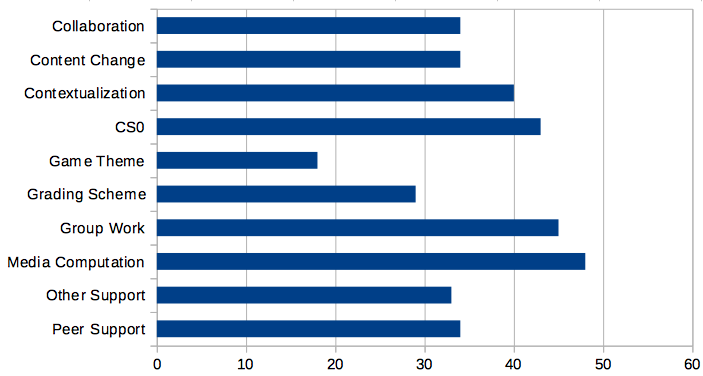
\includegraphics{../docs/fig/interventions.png}
\caption{Effectiveness of Interventions}
\label{f:pck-interventions}
\end{figure}

This list highlights the importance of cooperative learning.
\cite{Beck2013} looked at this specifically over three academic years
in courses taught by two different instructors, and found significant
benefits overall and for many subgroups: they not only had higher
grades, they left fewer questions blank on the final exam, which
indicates greater self-efficacy and willingness to try to debug
things.

As noted earlier, writing code isn't the only way to teach people how
to program.  \cite{Shel2017} reports that having novices work on
computational creativity exercises improves grades at several levels.
A typical exercise is to identify an everyday object (such as nail
clipper, a paper clip, Scotch tape) and describe the object in terms
of its inputs, outputs and functions.  This kind of teaching is
sometimes called ``unplugged''; the
\href{https://csunplugged.org/en/}{CS Unplugged} site has a collection
of lessons and exercises for doing this.

\section{Exercises}\label{s:pck-exercises}

\exercise{Checking for Common Errors}{individual}{20}

This list of common errors is taken from \cite{Sirk2012}.  Pick three,
and write an exercise for each to check that learners \emph{aren't}
making that mistake.

\begin{description}

  \item[Inverted assignment:] The student assigns the value of the
    left-hand variable to the right-hand side variable, rather than
    the other way around.

  \item[Wrong branch:] Even though the conditional evaluates to
    \texttt{False}, the student jumps to the \texttt{then} clause.

  \item[Wrong \texttt{False}:] As soon as the conditional evaluates to
    \texttt{False} , the student returns \texttt{False} from the
    function.
  
  \item[Executing function instead of defining it:] The student
    believes that a function is executed as it is defined.

  \item[Unevaluated parameters:] The student believes the function
    starts running before the parameters have been evaluated.

  \item[Parameter evaluated in the wrong frame:] The student creates
    parameter variables in the caller's frame, not in the callee's.

  \item[Failing to store return value:] The student does not assign
    the return value in the caller.

  \item[Assignment copies object:] The student creates a new object
    rather than copying a reference.

  \item[Method call without subject:] The student tries to call a
    method from a class without first creating an instance of the
    class.

\end{description}

\exercise{Mangled Code}{pairs}{15}

\cite{Chen2017} describes exercises in which students reconstruct code
that has been mangled by removing comments, deleting or replacing
lines of code, moving lines, inserting extra unneeded lines, and so
on.  Student performance on these correlates strongly with performance
on assessments in which students write code (i.e., whatever
traditional assignments are measuring, these are measuring as well),
but these questions require less (in-person) work to mark.  Take the
solution to a programming exercise you've created in the past, mangle
it in two different ways, and swap with a partner.

\exercise{The Rainfall Problem}{pairs}{10}

\cite{Solo1986} introduced the Rainfall Problem: write a program that
repeatedly reads in positive integers until it reads the integer
99999. After seeing 99999, the program should print out the average of
the numbers seen.  This problem has been used in many subsequent
studies of programming \cite{Fisl2014,Simo2013,Sepp2015}.

Solve the Rainfall Problem in the programming language of your
choice. Compare your solutions with those of your partner.

\exercise{Roles of Variables}{pairs}{15}

Take a short program you have written (5--15 lines) and classify each
of its variables using the categories defined in
\secref{s:pck-programming}.  Compare your classifications with those
of a partner: where did you agree? When you disagreed, did you
understand each other's view?

\exercise{Choose Your Own Adventures}{individual}{10}

Which of the three approaches described in \cite{Sorv2014}
(\secref{s:pck-now}) do you use when teaching? Or is your approach
best described in some other way?

\exercise{What Are You Teaching?}{individual}{10}

Compare the topics you teach to the list developed in \cite{Luxt2017}
(\secref{s:pck-now}).  Which topics do you cover?  What extra topics
do you cover that aren't in their list?

\exercise{Beneficial Activities}{individual}{10}

Look at the list of interventions developed by \cite{Viha2014}
(\secref{s:pck-help}).  Which of these things do you already do in
your classes?  Which ones could you easily add?  Which ones are
irrelevant?

\exercise{Visualizations}{individual}{10}

What visualization do you most like to use when teaching?  Is it a
static image or an animation?  Do you show it to your learners, do
they discover it on their own, or something in between?

\exercise{Misconceptions and Challenges}{small groups}{15}

The \href{http://www.pd4cs.org/}{Professional Development for CS
  Principles Teaching} site includes
\href{http://www.pd4cs.org/mc-index/}{a detailed list of student
  misconceptions and exercises}.  Working in small groups, choose one
section (such as data structures or functions) and go through their
list.  Which of these misconceptions do you remember having when you
were a learner?  Which do you still have?  Which have you seen in your
learners?
